\chapter{Chebyshev flow number of snarks} % chapter* je necislovana kapitola
\label{ch:bounds}

In this chapter, we prove a lower bound on the Chebyshev flow number of snarks depending on its order, with $5$ examples achieving the equality. Although we do not find an infinite class of snarks proving this bound is tight,  we construct a class of graphs, where only two vertices are of degree different from $3$, where their flow number corresponds to the bound for the order of this graph. Hence, these graphs might be good starting points for constructing the infinite class attaining the bound. Moreover, we show that these graphs can be adjusted to snarks with a smaller flow number, and hence, a snark with arbitrarily small flow number exists. Finally we construct a Chebyshev flow on generalised Blanuša snarks.

\section{Lower bound}

In one-dimensional flows, there has been proved a lower bound on the flow number of a snark 
\begin{equation*}
	\Phi_1(G) \geq 4 + \left.1\middle/\left\lceil\frac{n-4}{8}\right\rceil\right.
\end{equation*}
depending on the number $n$ of its vertices \cite[p. 14]{cycle_rank}. Moreover, there is also a meaningful lower bound on the two-dimensional Chebyshev flow number of the Petersen graph $P$ \cite[p. 99]{gloria_phd}. It states that $\Phi_2^\infty(P)\geq 5/2$. We provide a generalisation of this bound for any snark. Additionally, the bounding number is roughly a half of the bounding number in one dimension.

\begin{proposition} \emph{\cite[pp. 15, 16]{preprint}}
	Let $G$ denote a snark of order $n$. Then $\Phi_2^{\infty}(G) \geq 2+1 / \xi$, where $\xi=\left\lfloor\frac{n-2}{4}\right\rfloor$. \label{prop:lower_bound}
\end{proposition}

\begin{proof}
    
    For the sake of contradiction assume that $G$ admits a $2$D Chebyshev NZ flow $\varphi$ such that each edge $e \in E(G)$ satisfies $\varphi(e) = (\varphi_1(e), \varphi_2(e))$, $\|\varphi(e)\|_\infty\geq 1$, and $|\varphi_i(e)|<1+1/\xi$ for $i\in\{1, 2\}$.

    We call an edge $e \in E(G)$ \emph{large} with respect to $\varphi_i$ if $|\varphi_i(e)|\geq 1$, and \emph{small} otherwise. Observe that an edge $e$ can be large with respect to both $\varphi_1$ and $\varphi_2$, but it cannot be small with respect to both $\varphi_1$ and $\varphi_2$, since otherwise $\|\varphi(e)\|_\infty<1$.

    For $i\in\{1, 2\}$, denote by $S_i$ and $L_i$ the subgraphs of $G$ induced by the small and large edges with respect to $\varphi_i$, respectively. WLOG $|S_1| \leq |S_2|$. Moreover, from the previous observation, $S_1, S_2$ are disjoint, and hence $|S_1|\leq\left\lfloor\frac{1}{2}|E(G)|\right\rfloor=\left\lfloor\frac{3n}4\right\rfloor$.
    
    % From the previous observation, either $S_1$ or $S_2$ has at most $\lfloor|E(G)|/2\rfloor=\left\lfloor\frac{3n}4\right\rfloor$ edges, say $S_1$.
    \renewcommand{\qedsymbol}{$\blacksquare$}
    \begin{claim}
        $S_1$ contains no vertex of degree $3$. \label{clm:structure}
    \end{claim}
    \begin{proof}
        For the sake of contradiction, assume a vertex $v$ surrounded by three small edges w.r.t. $1$. Then, vertex $v$ must be surrounded also by three large edges w.r.t. $2$. Denote by $d_1, d_2, d_3$ the darts going out of $v$. WLOG $\varphi_{2}(d_1)\geq \varphi_{2}(d_2)\geq 0\geq\varphi_{2}(d_3)$. Then, the flow conservation requires
        \begin{equation*}
            0 = \varphi_2(d_1) + \varphi_2(d_2) + \varphi_2(d_3) \geq 1 + 1 + (-1-1/\xi) = 1-1/\xi,
        \end{equation*}
        which is equivalent to $\xi\leq 1$, and hence $n\leq 9$. But there are no snarks with less than $10$ vertices, a contradiction.
        % Observe that $\Delta(L_i) \leq 2$, because the sum of three real numbers all with absolute value in the interval $[1, 1+1/\xi)$ cannot give $0$ as a result, making the Kirkoff's law impossible to be satisfied by $\varphi$ around a vertex of $G$. Hence $S_i$ is spanning, for otherwise $\Delta(L_i) = 3$ and $\Delta(S_i) \leq 2$, for otherwise $\Delta(L_{3-i}) = 3$.
    \end{proof}

    \begin{claim}
        If $C\subseteq E(L_i)$ is an odd edge-cut of $G$ for any $i\in\{1,2\}$, then $|C|\geq 2\xi+3$. \label{clm:cut}
    \end{claim}
    \begin{proof}
        Consider an odd edge-cut $C$ of $G$ containing $2k+1$ large edges w.r.t. $i$ separating components $G_1, G_2$. Denote the corresponding darts from $G_1$ to $G_2$ as $d_1,d_2,\dots,d_{2k+1}$. WLOG assume that $\varphi_i(d_j) \geq 0$ for all $1\leq j\leq k+1$. Then, the generalised flow conservation requires that
        \begin{equation*}
            0=\sum_{j=1}^{2k+1} \varphi_i(d_j) = \sum_{j=1}^{k+1} \varphi_i(d_j) + \sum_{j=k+2}^{2k+1} \varphi_i(d_j) > (k+1)\cdot 1 + k\cdot(-1-1/\xi) = 1-k/\xi,
        \end{equation*}
        which is equivalent to $k>\xi$.
    \end{proof}

    \begin{claim}
        A path of length $2k$ with $k<\xi$ cannot be a component of $S_1$. \label{clm:path}
    \end{claim}
    \begin{proof}
        For the sake of contradiction assume that $S_1$ contains a path of length $2k$ with $k<\xi$. Then the edges adjacent to this path are in $L_1$ and they form an odd edge-cut of $G$, containing at most $2k+3<2\xi+3$ edges, which is in contradiction with Claim \ref{clm:cut}.
    \end{proof}

    \begin{claim}
        A cycle of length $2k+1$ with $k\leq\xi$ cannot be a component of $S_1$. \label{clm:cycle}
    \end{claim}
    \begin{proof}
        For the sake of contradiction assume that $S_1$ contains a cycle of length $2k+1$ with $k\leq\xi$. Then the edges adjacent to this cycle are in $L_1$ and they form an odd edge-cut of $G$, containing at most $2k+1\leq 2\xi+1<2\xi+3$ edges, which is in contradiction with Claim \ref{clm:cut}.
    \end{proof}

    \begin{claim}
        $S_1$ cannot contain a perfect matching of $G$. \label{clm:matching}
    \end{claim}
    \begin{proof}
        For the sake of contradiction assume that $S_1$ contains a perfect matching $M$ of $G$. Then also $L_2$ contains $M$. Next, $F=E(G)\setminus M$ is a $2$-factor of $G$. Since $G$ is a snark, its oddness is at least two, and therefore, $F$ contains at least two odd cycles. Then, the smallest one has length $2k+1\leq\frac n2$. It follows that $k\leq\frac{n-2}{4}$, and since $k$ is natural, we also have $k\leq\left\lfloor\frac{n-2}{4}\right\rfloor=\xi$. Then the edges adjacent to this cycle are in $L_2$, and they form an odd edge-cut of $G$, containing at most $2k+1\leq 2\xi+1$ edges, which is in contradiction with Claim \ref{clm:cut}.
        % Note that $F$ must contain an odd cycle of length $2k+1\leq\frac n2$ \textcolor{red}{explain more -- here's implicitly used that $G$ is snark}. 
    \end{proof}

    By Claim \ref{clm:structure} we know that $S_1$ contains only paths and cycles. Note that by Claim \ref{clm:path}, each even path in $S_1$ contains at least $2\xi$ edges. Similarly by Claim \ref{clm:cycle}, each odd cycle in $S_1$ contains at least $2\xi+3$ edges. Let \emph{odd components} denote odd cycles and even paths. We aim to show that $S_1$ has less than two odd components. Otherwise,
    \begin{equation}
    	\left\lfloor\frac{3n}{4}\right\rfloor \geq E(S_1) \geq 4\xi=4\left\lfloor\frac{n-2}{4}\right\rfloor.\label{eq:lower_bound_two_odd_components}
    \end{equation}
    We disprove this inequality by induction. For $n\in\{10, 20\}$ clearly $\left\lfloor\frac{3n}{4}\right\rfloor<4\left\lfloor\frac{n-2}{4}\right\rfloor$. Increasing the order $n$ by $4$ results in increasing the LHS and RHS by $3$ and $4$, respectively. Hence, the \eqref{eq:lower_bound_two_odd_components} holds for no even $n\geq 10$ except $12$ and $16$. However, there are no snarks of order $12$, $16$ or smaller than $10$, a contradiction.
    
    Therefore, $S_1$ contains at most one odd component. On the other hand, $S_1$ has even order, so it contains even number of odd components. As a result, $S_1$ contains no odd component, so it consists only of odd paths and even cycles. These also induce a perfect matching of $G$, but that is in contradiction with Claim \ref{clm:matching}.
    \renewcommand{\qedsymbol}{$\square$}
\end{proof}

For now, we are aware of five snarks meeting this bound – Petersen graph $P$ with the flow number $5/2$, both Blanuša snarks $B_2^{(1)}, B_2^{(2)}$ with flow numbers $9/4$ (which is a part of more general result in Proposition \ref{prop:blanusa_chnzf}) and $2$ out of $6$ snarks on $20$ vertices with flow numbers also equal to $9/4$. From computational results, we know that no other example of tightness exists on at most $26$ vertices \cite[p. 17]{preprint}. Although we do not know about any other snark meeting this bound, we think the bound is not so far from reality, since we found an infinite class of graphs that are nearly cubic and meet this bound.

\section{Petersen book graphs}

The mentioned class was already introduced when constructing graphs with given circular flow number \cite[p. 312]{given_flow_number_not_snarks}.
\begin{definition}
Let $Q$ be the Petersen graph without an edge (since the Petersen graph is edge-transitive, it does not matter which one is removed) and denote its two vertices of degree two by $x$ and $y$. Then, a \emph{Petersen book $PB_n$} is a graph, which arises from $n$ copies of $Q$ by identifying all vertices corresponding to $x$ in a vertex $\hat{x}$, similarly all vertices corresponding to $y$ in $\hat{y}$ and finally joining $\hat{x}$ and $\hat{y}$ by an edge.
\end{definition}

\begin{figure}[h!]
\centering
\begin{subfigure}{0.45\textwidth}
\centering
\input images/pf2.tex
\caption{$n=2$}
\end{subfigure}
\begin{subfigure}{0.45\textwidth}
\centering
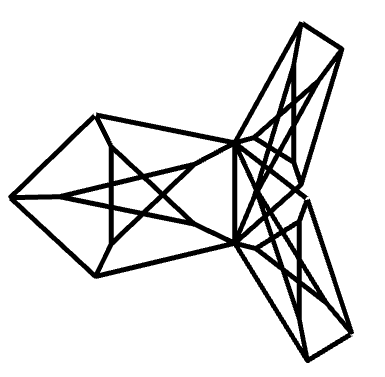
\includegraphics[height=35mm]{images/pf3.png}
\caption{$n=3$}
\end{subfigure}
\caption{Two small examples of $PB_n$ graphs}
\end{figure}

\begin{lemma} \emph{\cite[p. 312]{given_flow_number_not_snarks}}
For each positive integer $n$, $\Phi_1(PB_n)=4+1/n$.
\end{lemma}

From Proposition \ref{prop:nzf_from_flow_pair}, one can easily see, that if $PB_n$ admits a $t$-flow-pair, then $t\geq 1/(2n)$. And for $t=1/(2n)$, the flow-pair also exists.

\begin{proposition}
For each positive integer $n$, $PB_n$ admits a $(1/(2n))$-flow-pair.
\end{proposition}
\begin{proof}
In Figure \ref{fig:Q_flow}, we define flow values of flow-pair $(\varphi_1, \varphi_2)$ on one copy of $Q$. The edges of the $2$-factor induced by $\varphi_1$ are in bold.
\begin{figure}[h!]
\centering
\input images/pf_construction.tex
\caption{$(1/(2n))$-flow-pair on $Q$}
\label{fig:Q_flow}
\end{figure}
We can check that in each vertex except $x$ and $y$, the flow conservation constraint is satisfied, and non-bolded edges use only flow values $2n$ and $2n+1$. Hence, all flow values used in one copy of $Q$ are feasible. Moreover, when we join $n$ copies of $Q$, the sum of flow values outgoing from $\hat{x}$ will be $(0, 2n)$, and the same will be the sum of flow values ingoing to $\hat{y}$. However, this is also a feasible flow value, so by setting $\varphi\left(\vv{\hat{y}\hat{x}}\right) = (0, 2n)$, we get the desired $1/(2n)$-flow-pair of $PB_n$.
\end{proof}

This Proposition also gives an upper bound on the Chebyshev flow number of $PB_n$.
\begin{corollary}
For each positive integer $n$, $\Phi_2^\infty(PB_n)\leq 2+1/(2n)$.
\end{corollary}

By a computer, we verified that $\Phi_2^\infty(PB_3)=2+1/6$ and $\Phi_2^\infty(PB_4)=2+1/8$, so we expect that the inequality can be replaced by the equality.

\begin{conjecture}
For each positive integer $n$, $\Phi_2^\infty(PB_n) = 2+1/(2n)$.
\end{conjecture}

Note that $PB_n$ is of order $8n+2$. Even though $PB_n$ is not cubic for $n\geq 2$ (due to two vertices of degree $2n+1$), observe that by inserting the order into the bound from Proposition \ref{prop:lower_bound}, we get $1/(2n)$. Therefore, if we were able to split each of the two vertices of degree $2n+1$ into vertices of degree $2$ and one vertex of degree $3$ without increasing the flow number or creating a $3$-edge-colourable graph, after smoothing vertices of degree $2$, we will obtain a graph meeting the lower bound.

This is possible for $n=2$, where we can obtain both Blanuša snarks. For $n=3$, we already know this is not possible, because all snarks on $26$ vertices have 2D Chebyshev flow number at least $2+1/4$. However, we are able to reduce the degrees of these vertices so that in the resulting graph, only one vertex is not of degree $3$, and its degree is $5$. Then we replaced this vertex by a $5$-cycle. By computer, we verified that the flow number still remains the same, and so we constructed a snark on $30$ vertices with 2D Chebyshev flow number $2+1/6$. Hence, we suspect, no snark with 2D Chebyshev flow number $2+1/6$ on $28$ vertices exists.

In summary, adjusting $PB_n$ without changing the flow number can lead to snarks with Chebyshev flow number near the proved bound. Now we will show one general construction, giving an upper bound on the order of the graph with sufficiently small flow number. This method is inspired by a similar construction for circular flow number \cite[pp. 193-195]{given_flow_number}.

\begin{proposition}
Let $G$ be a graph with a $p/q$-flow-pair. Then there exists a cubic graph $G'$ with a $p/q$-flow-pair.
\end{proposition}
\begin{proof}
Fix a $p/q$-flow-pair of $G$ and consider a vertex $v$ with degree $d$ greater than $3$. We aim to construct a cubic $d$-pole, which will be the replacement of $v$ in $G$. Therefore, the multiset of the flow values on dangling edges of this pole should be the same as the multiset of flow values surrounding $v$ in the original graph.

Let us start with the $d$ dangling edges with corresponding flow values. Now, we attach graphs to the dangling edges, to obtain only dangling edges with flow values $(0, \pm(p+q)), (\pm 1, 0)$ in the end. To get rid of unwanted edges with zero first coordinate and $a>0$, we will use the graph in Figure \ref{fig:network0}. The graph for $a<0$ can be obtained in a similar manner.
\begin{figure}[h!]
 \captionsetup{labelsep=none}
 \centering 
 \input images/redirecting_vertex.tex
 \caption{}
 \label{fig:network0}
\end{figure}

So now we are left with the unwanted edges with a non-zero first coordinate. Take two dangling edges with first coordinates equal to $1$ and second coordinates $-p-q < a \leq b < p+q$. Let $x=\min\{p+q-b, p+q+a\}$. We attach $\lfloor x/p\rfloor$ copies of the graph in Figure \ref{fig:network1} with $\delta=p$ and then another copy with $\delta=x\mod p$. This causes we get either $(1, -p-q)$ or $(1, p+q)$ on one of the dangling edges. To this dangling edge, we can attach dangling edges with flow values $(1, 0)$ and $(0, \pm(p+q))$, and hence reduce the number of unwanted edges. Since this can be done while there are at least two dangling edges with the first coordinate equal to $1$, we will end up with at most one conflicting edge, whose first coordinate of flow value is $1$. By a similar reasoning, we can deal with dangling edges, where the first coordinate of the flow value is $-1$.

\begin{figure}[h!]
 \captionsetup{labelsep=none}
 \centering
 \input images/redirecting_network.tex
 \caption{}
 \label{fig:network1}
\end{figure}

At this moment, the majority of dangling edges have flow values $(\pm 1, 0)$ and $(0, \pm(p+q))$. The only two possible exceptions are $(1, s)$ and $(-1, t)$ for some $-p-q < s, t < p+q$. From the flow conservation constraint, we deduce that $s+t\equiv 0\pmod{p+q}$. If $s+t=0$, we can attach those dangling edges and smooth their common vertex of degree $2$. On the other hand, if $s+t=\pm(p+q)$, we will additionally attach a $(0, \pm(p+q))$ dangling edge to fulfill the flow conservation constraint.
As the last step, we realize, that from the flow conservation constraint, the number of $(1, 0)$ dangling edges is equal to the number of $(-1, 0)$ dangling edges (and same for the $(0, \pm(p+q))$ edges), so we can attach edges with opposite flow values and smooth their common vertex. Finally, we ended up with (not necessarily connected) cubic $d$-pole with desired properties, and hence, we constructed a cubic graph with $p/q$-flow-pair.
\end{proof}

\begin{corollary}
For any $r>2$, there exists a non-colourable cubic graph whose 2D Chebyshev flow number is at most $r$.
\end{corollary}
\section{Generalised Blanuša snarks}
\label{sec:blanusa_construction}

Now, we move to generalised Blanuša snarks. In one dimension, the flow number of generalised Blanuša snarks is proved to be $4+1/2$. The paper concerning these graphs also shows an explicit construction of the circular flow \cite[p. 978]{blanusa_flow_number}. We modify this construction and construct a $1/4$-flow-pair. From this, we know that all generalised Blanuša snarks have the 2D Chebyshev flow number at most $2+1/4$.

\begin{figure*}[h!]
\begin{subfigure}{\textwidth}
\centering
\input images/generalised_blanusa_type_I.tex
\caption{of type I}
\label{fig:FP_first_blanusa}
\end{subfigure}
\begin{subfigure}{\textwidth}
\centering
\input images/generalised_blanusa_type_II.tex
\caption{of type II}
\label{fig:FP_second_blanusa}
\end{subfigure}
\caption{A $1/4$-flow-pair on generalised Blanuša snarks}
\end{figure*}

\begin{proposition}
For each $n\geq 2$, both $B_n^{(1)}$ and $B_n^{(2)}$ have a ChNZ $9/4$-flow. \label{prop:blanusa_chnzf}
\end{proposition}
\begin{proof}
In Figures \ref{fig:FP_first_blanusa} and \ref{fig:FP_second_blanusa}, we illustrate the $1/4$-flow-pairs $\varphi=(\varphi_1, \varphi_2)$ on generalised Blanuša snarks, where the edges of the $2$-factor induced by $\varphi_1$ are in bold. Then, from Proposition \ref{prop:nzf_from_flow_pair}, these graphs have a ChNZ $9/4$-flow.
\end{proof}

From Proposition \ref{prop:lower_bound}, we know that $\Phi_2^\infty\big(B_2^{(1)}\big)=\Phi_2^\infty\big(B_2^{(2)}\big)\geq 9/4$, so for the two Blanuša snarks, the bound meets the construction. For generalised Blanuša snarks on $26$ and $34$ vertices, we verified by computer that their 2D Chebyshev flow number is $9/4$. Therefore, we suspect it holds in general.
\begin{conjecture}
For each $n\geq 2$, $\Phi_2^\infty\big(B_n^{(1)}\big)=\Phi_2^\infty\big(B_n^{(2)}\big) = 9/4$.
\end{conjecture}